\section{\systemname\ Architecture}
\label{sec:design}

\systemname\ treats expert precision as an online, budget-constrained resource. Each expert has prepared lower- and higher-precision host representations, denoted $b^{\text{lo}}$ and $b^{\text{hi}}$. Exactly one representation is published for device dispatch; a bounded staging copy may coexist only while a transition is in flight. The runtime changes which experts occupy $b^{\text{hi}}$ subject to three constraints: (C1)~budget feasibility, (C2)~no explicit transition synchronization on the forward path, and (C3)~stability under routing fluctuations.

\begin{figure*}[t]
    \centering
    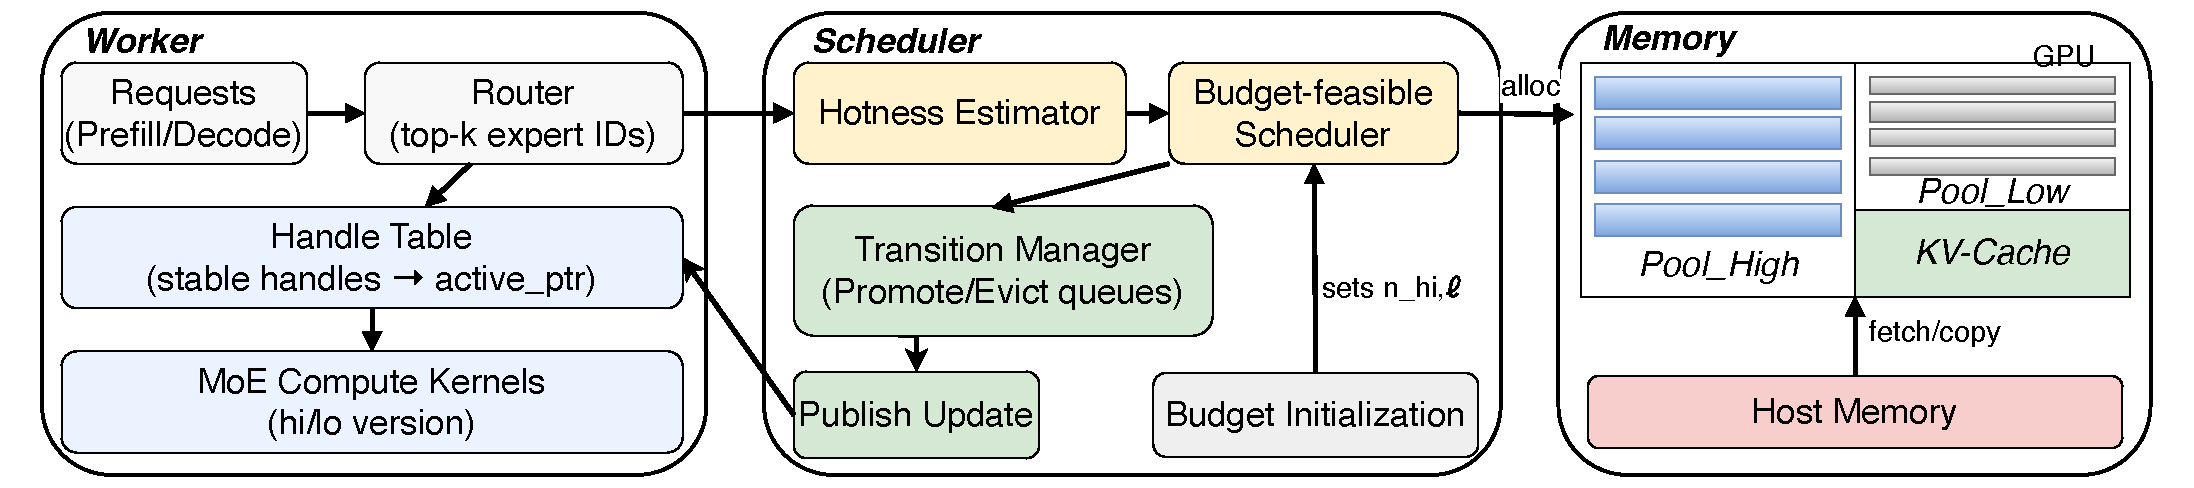
\includegraphics[width=0.93\linewidth]{figures/dynaexq_arch.pdf}
    \caption{System architecture of \systemname. The worker resolves a versioned expert handle; a scheduler observes router traces and updates precision residency under a strict HBM budget; a transition pipeline carries out promotions and demotions on a dedicated migration stream.}
    \label{fig:architecture_overview}
    \vspace{-1em}
\end{figure*}

\subsection{Architecture Overview and Execution Model}
\label{sec:overview}

\autoref{fig:architecture_overview} shows the end-to-end control loop. The design separates \emph{policy} (what to change) from \emph{mechanisms} (how to change safely).

\paragraph{Policy.}
The scheduler interprets router-derived traffic and chooses a budget-feasible high-precision resident set per layer: hotness estimation via periodic aggregation, top-$n$ selection under fixed per-layer capacities, and hysteresis to damp oscillation. It emits target sets and promotion/demotion candidates but does not allocate GPU memory directly.

\paragraph{Mechanisms.}
Three mechanisms implement this runtime execution model:
(i)~versioned, representation-immutable per-expert handles with publish-after-complete semantics isolate dispatch from in-flight data movement;
(ii)~partitioned device pools and a budget tracker admit or reject each transition before any allocation;
(iii)~an asynchronous transition pipeline runs data movement on a dedicated CUDA stream and publishes a new handle only after transfer completes.
Consequently, transition submission does not wait for a copy, dispatch cannot observe a partially populated buffer, and no transition starts without a prior reservation against the declared HBM envelope. Stream separation does not eliminate memory-bandwidth contention, which we measure end to end.

\paragraph{Worker-side dispatch.}
On the worker side, each request invokes the router to obtain top-$k$ expert IDs. Each ID resolves to a versioned handle containing a fully materialized device block and its quantization metadata. Dispatch observes either the previous complete handle or the next complete handle; it does not mutate a handle in place.

\paragraph{Scheduler-side control.}
The scheduler consumes router traces asynchronously. Per-expert hotness statistics feed a budget-feasible selection that determines, for each layer~$\ell$, a high-precision resident set subject to a layer capacity $n_{\mathrm{hi},\ell}$. The resulting target sets drive a transition manager that maintains promote/evict queues and issues background work on a migration stream.

\paragraph{Budget initialization.}
Before inference, the system derives per-layer capacities $\{n_{\mathrm{hi},\ell}\}$ from total device memory $M_{\text{total}}$. Let $M_{\text{fixed}}$ reserve non-expert parameters, activations, KV cache, conversion workspace, and a safety margin. Let $M_{\text{trans}}$ be preallocated headroom for at most $K$ simultaneous publish-before-reclaim transitions, and let $m^{\text{hi}}_\ell$ and $m^{\text{lo}}_\ell$ be the measured packed bytes of one expert at each tier in layer~$\ell$. Initialization chooses capacities satisfying
\begin{equation}
\begin{aligned}
M_{\text{resident}}
&=\sum_{\ell}\!\left[n_{\mathrm{hi},\ell}m^{\text{hi}}_\ell+
(E_{\ell}-n_{\mathrm{hi},\ell})m^{\text{lo}}_\ell\right],\\
M_{\text{trans}}
&=K\max_{\ell,b\in\{\mathrm{hi},\mathrm{lo}\}}m^b_\ell,\\
M_{\text{resident}}+M_{\text{trans}}
&\le M_{\text{total}}-M_{\text{fixed}}.
\end{aligned}
\label{eq:hbm-budget}
\end{equation}
where $E_\ell$ is the routed-expert count in layer~$\ell$. The implementation supports uniform, expert-count-proportional, and greedy capacity allocation; the evaluation uses deterministic proportional allocation. An independent train/validation calibration trace first runs the all-low configuration and ranks experts by mean routed probability mass across prompts. This FP64 accumulator is order-invariant, unlike the online EMA, and avoids initializing from an arbitrary expert-ID prefix. The first $n_{\mathrm{hi},\ell}$ ranked experts populate the initial higher-precision set; sensitivity experiments vary only this prefix length. Each artifact binds the checkpoint, calibration-source hash, selected prompt identifiers, aggregation rule, ranking hash, and clean code revision. After initialization, $n_{\mathrm{hi},\ell}$ remains fixed and only expert \emph{identities} change online.

\paragraph{Scope of the memory invariant.}
Equation~\eqref{eq:hbm-budget} is enforced exactly for memory owned by \systemname: resident expert blocks, staging blocks, and conversion workspace are allocated or reserved at startup, and no transition is admitted beyond those capacities. The whole-process HBM cap additionally assumes that KV cache, activation, and framework allocations remain within their declared reservations. Startup checks available HBM against all declared components, but the prototype does not intercept a framework allocator if a later request exceeds its KV or activation reserve. We report both the expert-pool counters and the observed process peak to distinguish the enforced invariant from this deployment assumption.

\subsection{Online Scheduling Policy}
\label{sec:policy}

The scheduling policy determines which experts should occupy the limited high-precision capacity. It is kept simple so that its behavior is easy to reason about and its per-tick cost stays small relative to inference.

\paragraph{Hotness estimation.}
For a forward step with $N_\ell$ routed token positions, let $p_{\ell,t,e}$ be the router probability for expert $e$ when it is selected in the top-$k$ set $\mathcal{R}_{\ell,t}$, and zero otherwise. The runtime uses the selected probability mass per token,
\[
c_{\ell,e}=\frac{1}{N_\ell}\sum_{t=1}^{N_\ell}
\mathbf{1}[e\in\mathcal{R}_{\ell,t}]\,p_{\ell,t,e}.
\]
Thus the signal captures both selection frequency and router confidence. Updates are applied after every observation, with $c_{\ell,e}=0$ for unselected experts so stale scores decay. Residency decisions are triggered every $T_u$ forward steps; the step-based definition is deterministic under replay and makes the number of router observations per decision explicit. The smoothed hotness score is:
\[
S_{\ell,e} \leftarrow \alpha \cdot S_{\ell,e} + (1-\alpha)\cdot c_{\ell,e},
\]
where $\alpha \in [0,1)$ controls how quickly past observations decay. This construction uses router outputs only and requires no labels or online quality signals.

\paragraph{Budget-feasible selection.}
For each layer $\ell$ with capacity $n_{\mathrm{hi},\ell}$, the high-precision set is:
\[
H_\ell \leftarrow \mathrm{TopN}\!\left(\{S_{\ell,e}\}_e,\; n_{\mathrm{hi},\ell}\right).
\]
Selection is local to each layer and budget-feasible by construction: no cross-layer coordination is needed. The set difference against the current resident set yields promotion candidates $H_\ell \setminus H_\ell^{\mathrm{cur}}$ and demotion candidates $H_\ell^{\mathrm{cur}} \setminus H_\ell$. These candidates are passed to the transition pipeline, which admits promotions only when the budget tracker can reserve the required memory (Section~\ref{sec:memmgmt}).

\paragraph{Hysteresis for stability.}
A plain top-$N$ rule can cause unnecessary churn when several experts have similar hotness scores. Each swap triggers a promotion and a matching demotion, consuming migration bandwidth without improving quality. We therefore apply additive-margin hysteresis: after the cold-start set reaches capacity, the highest-scoring outsider replaces the lowest-scoring incumbent only when their score difference exceeds $\delta$. Candidate pairs are processed in score order until the inequality fails. Hysteresis does not change the budget constraint; it reduces oscillations and makes the transition rate more predictable under transient routing fluctuations.

The policy produces a target set per layer at cadence $T_u$. A target does not become visible merely because it was selected: each expert dispatch continues to acquire the last published handle until that expert's pending version switch completes.

\subsection{GPU Memory Management}
\label{sec:memmgmt}

Dynamic residency stresses GPU memory in two ways. First, promotions and evictions allocate large weight buffers; if these share a general-purpose device heap with variable request sizes, external fragmentation and allocator jitter can inflate latency variance. Second, several transitions may overlap in time; if their aggregate footprint is unbounded, concurrent promotions can exhaust the device budget even when each is individually feasible.

\paragraph{Partitioned pools and fragmentation control.}
We divide the GPU memory assigned to expert weights into disjoint per-layer, per-tier pools: $\texttt{pool\_hi}$ for high-precision versions and $\texttt{pool\_lo}$ for low-precision versions. Their capacities are fixed independently of the logically reserved KV-cache and framework budgets. Within each pool, one fixed-size byte block stores one expert's measured packed representation. This eliminates variable-size external fragmentation and keeps the free/allocate path uniform, following the same principle as paged KV-cache memory in LLM inference engines~\cite{kwon2023vllm}. Each pool maintains its own free list, so transitions never invoke the general-purpose device allocator. Separating capacities by precision tier prevents churn in one tier from consuming blocks assigned to the other. Rapid promotions filling $\texttt{pool\_hi}$, for example, cannot encroach on $\texttt{pool\_lo}$'s resident set.

\paragraph{Budget model and admission.}
A \texttt{BudgetTracker} enforces the global memory budget through explicit reservation and release operations. The usable device memory $M_{\text{total}}$ is partitioned at startup into:
\begin{itemize}[leftmargin=1.5em, itemsep=0pt, topsep=2pt]
\item $M_{\text{fixed}}$: declared KV cache and activation reserves, measured non-expert model state, safety margin, and a conservative two-expert kernel-conversion workspace per admitted INT4 transition.
\item $M_{\text{exp,hi}}^{\text{cap}}$: cap on resident high-precision expert weights.
\item $M_{\text{exp,lo}}^{\text{cap}}$: cap on resident low-precision expert weights.
\item A global fixed-block staging pool for publish-before-reclaim overlap, so concurrent migration work is allocated and accounted for before it starts.
\end{itemize}
Every transition must call \texttt{try\_reserve} before entering the executor. Admission checks the destination-tier cap, the pending-transfer cap, and a cross-tier cap on all committed plus pending expert bytes. The scheduler emits a replacement as an indivisible pair and orders its demotion before its promotion; the global staging pool covers the publish-before-reclaim overlap. When the paired transition frees the destination layer's resident slot, the runtime copies any staging-backed handle into that slot and returns the transient block, preventing staging capacity from becoming long-lived residency. If admission or allocation fails, the request is rejected and reconsidered from the published state at a later tick. Because the device pools are preallocated and admission precedes allocation, concurrent requests cannot grow \systemname-owned HBM beyond the startup envelope.

\subsection{Asynchronous Transition Pipeline}
\label{sec:pipeline}

The transition pipeline performs data movement and pointer updates while the compute stream runs independently.

\paragraph{Versioned-handle publication.}
The registry maps each expert key to a versioned handle whose published representation fields (tier, block, and packed metadata) are never modified in place; only lease and last-use bookkeeping changes. Publication is a single dictionary replacement under the registry lock. Before issuing expert kernels, an adapter acquires a short read lease on the currently published object and releases it after recording the compute-stream event. A handle retains the latest event for each compute stream, bounding metadata by serving concurrency rather than request count. A monotonically increasing version lets adapters skip unchanged metadata refreshes. During promotion, the destination block is filled on the migration stream and the transition worker waits for its completion event before publishing the new handle. The reclaimer first waits for the old object's lease count to reach zero and then waits for all of its per-stream last-use events. This two-part fence covers the otherwise unsafe interval in which dispatch has read an old handle but has not yet launched its kernel.

\begin{figure}[t]
    \centering
    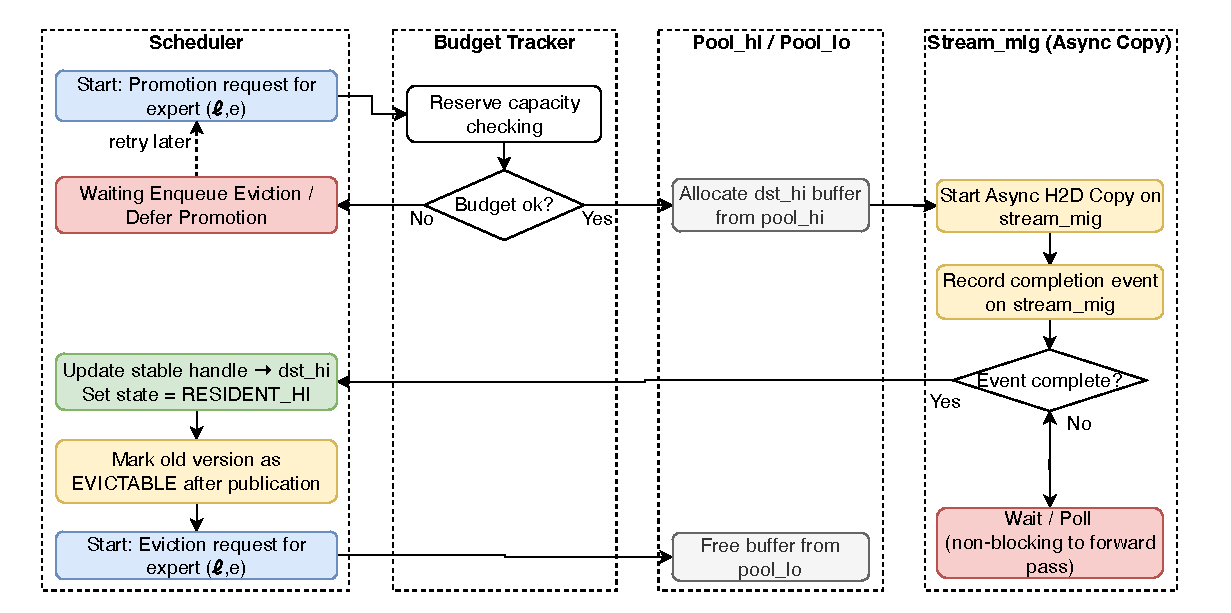
\includegraphics[width=0.99\columnwidth]{figures/dynaexq_procedure.pdf}
    \caption{Promotion and eviction procedure in the transition pipeline.}
    \label{fig:procedure}
    \vspace{-1em}
\end{figure}

\paragraph{Stream separation and backpressure.}
A bounded thread executor issues copies on a dedicated CUDA stream $\texttt{stream}_{\text{mig}}$, disjoint from the default compute stream used by attention and expert kernels. The scheduler keeps each replacement pair intact and submits its demotion first. Backpressure is implemented at admission: a request enters the executor only after passing the budget checks above. A rejected request is not reported as resident; the next decision is recomputed from a snapshot of actually published tiers.

\paragraph{Promotion procedure.}
For a target expert $(\ell,e)$, the pipeline proceeds as follows (\autoref{fig:procedure}):
\begin{enumerate}[leftmargin=1.5em, itemsep=0pt, topsep=2pt]
\item Obtain a successful \texttt{try\_reserve} for the high-precision footprint.
\item Allocate a destination buffer from $\texttt{pool\_hi}$, or from the bounded global staging pool if the resident slot is not yet reclaimable.
\item Issue an asynchronous copy from the pinned host representation on $\texttt{stream}_{\text{mig}}$.
\item Record a CUDA event on $\texttt{stream}_{\text{mig}}$.
\end{enumerate}
The registry publication executes only after the completion event fires, so dispatch never observes a partially populated buffer. The compute stream does not wait on the migration stream; a subsequent dispatch simply resolves the latest published handle.

\paragraph{Eviction procedure.}
When the scheduler marks an expert for demotion, the pipeline publishes the low-precision handle and then reclaims the high-precision buffer. The old handle's read leases close the read-before-launch race; its per-stream compute events then ensure no issued kernel is still reading the buffer before it returns to the pool.

\paragraph{Host-side weight preparation.}
Before timed inference, the prototype materializes both packed tiers in pinned host memory one layer at a time and releases that layer's native source parameters as soon as both versions are complete. This avoids holding the full source model and the full dual-tier cache simultaneously. It next populates every device-resident handle from the fixed pools. The untimed initialization still increases host DRAM demand but makes a measured transition a copy of an existing representation rather than first-use quantization. The experiment aborts if any expert cannot be cached, released, or registered; it never silently falls back to native weights.
